
\documentclass[12pt,a4paper]{article}
\usepackage[utf8]{inputenc}
\usepackage{graphicx}
\usepackage[dvipsnames]{xcolor}
\usepackage{tikz}
\usetikzlibrary{fit}
\usepackage{lmodern}
\usepackage{sectsty}
\usepackage{hyperref}
\usepackage[english]{babel}


\sectionfont{\color{OliveGreen}\fontfamily{lmss}\selectfont}
\subsectionfont{\fontfamily{lmss}\selectfont}

\begin{document}
   \begin{titlepage}
      {\fontfamily{lmss}\selectfont
      	\centering
      	
\includegraphics[width=0.40\textwidth]{logo.png}\par\vspace{1cm}
      	{\LARGE Subtrop \par}
      	\vspace{0.25cm}
      	{\huge\bfseries \color{OliveGreen}Harvest\par}
      	\vspace{1cm}
      	{\Large\textit{by} Brute Force\par}
         \vspace{0.25cm}
         \begin{tikzpicture}
            \node [inner sep=0pt,,outer sep=0pt,clip,rounded corners=0.5cm] (pict) at (0,0) {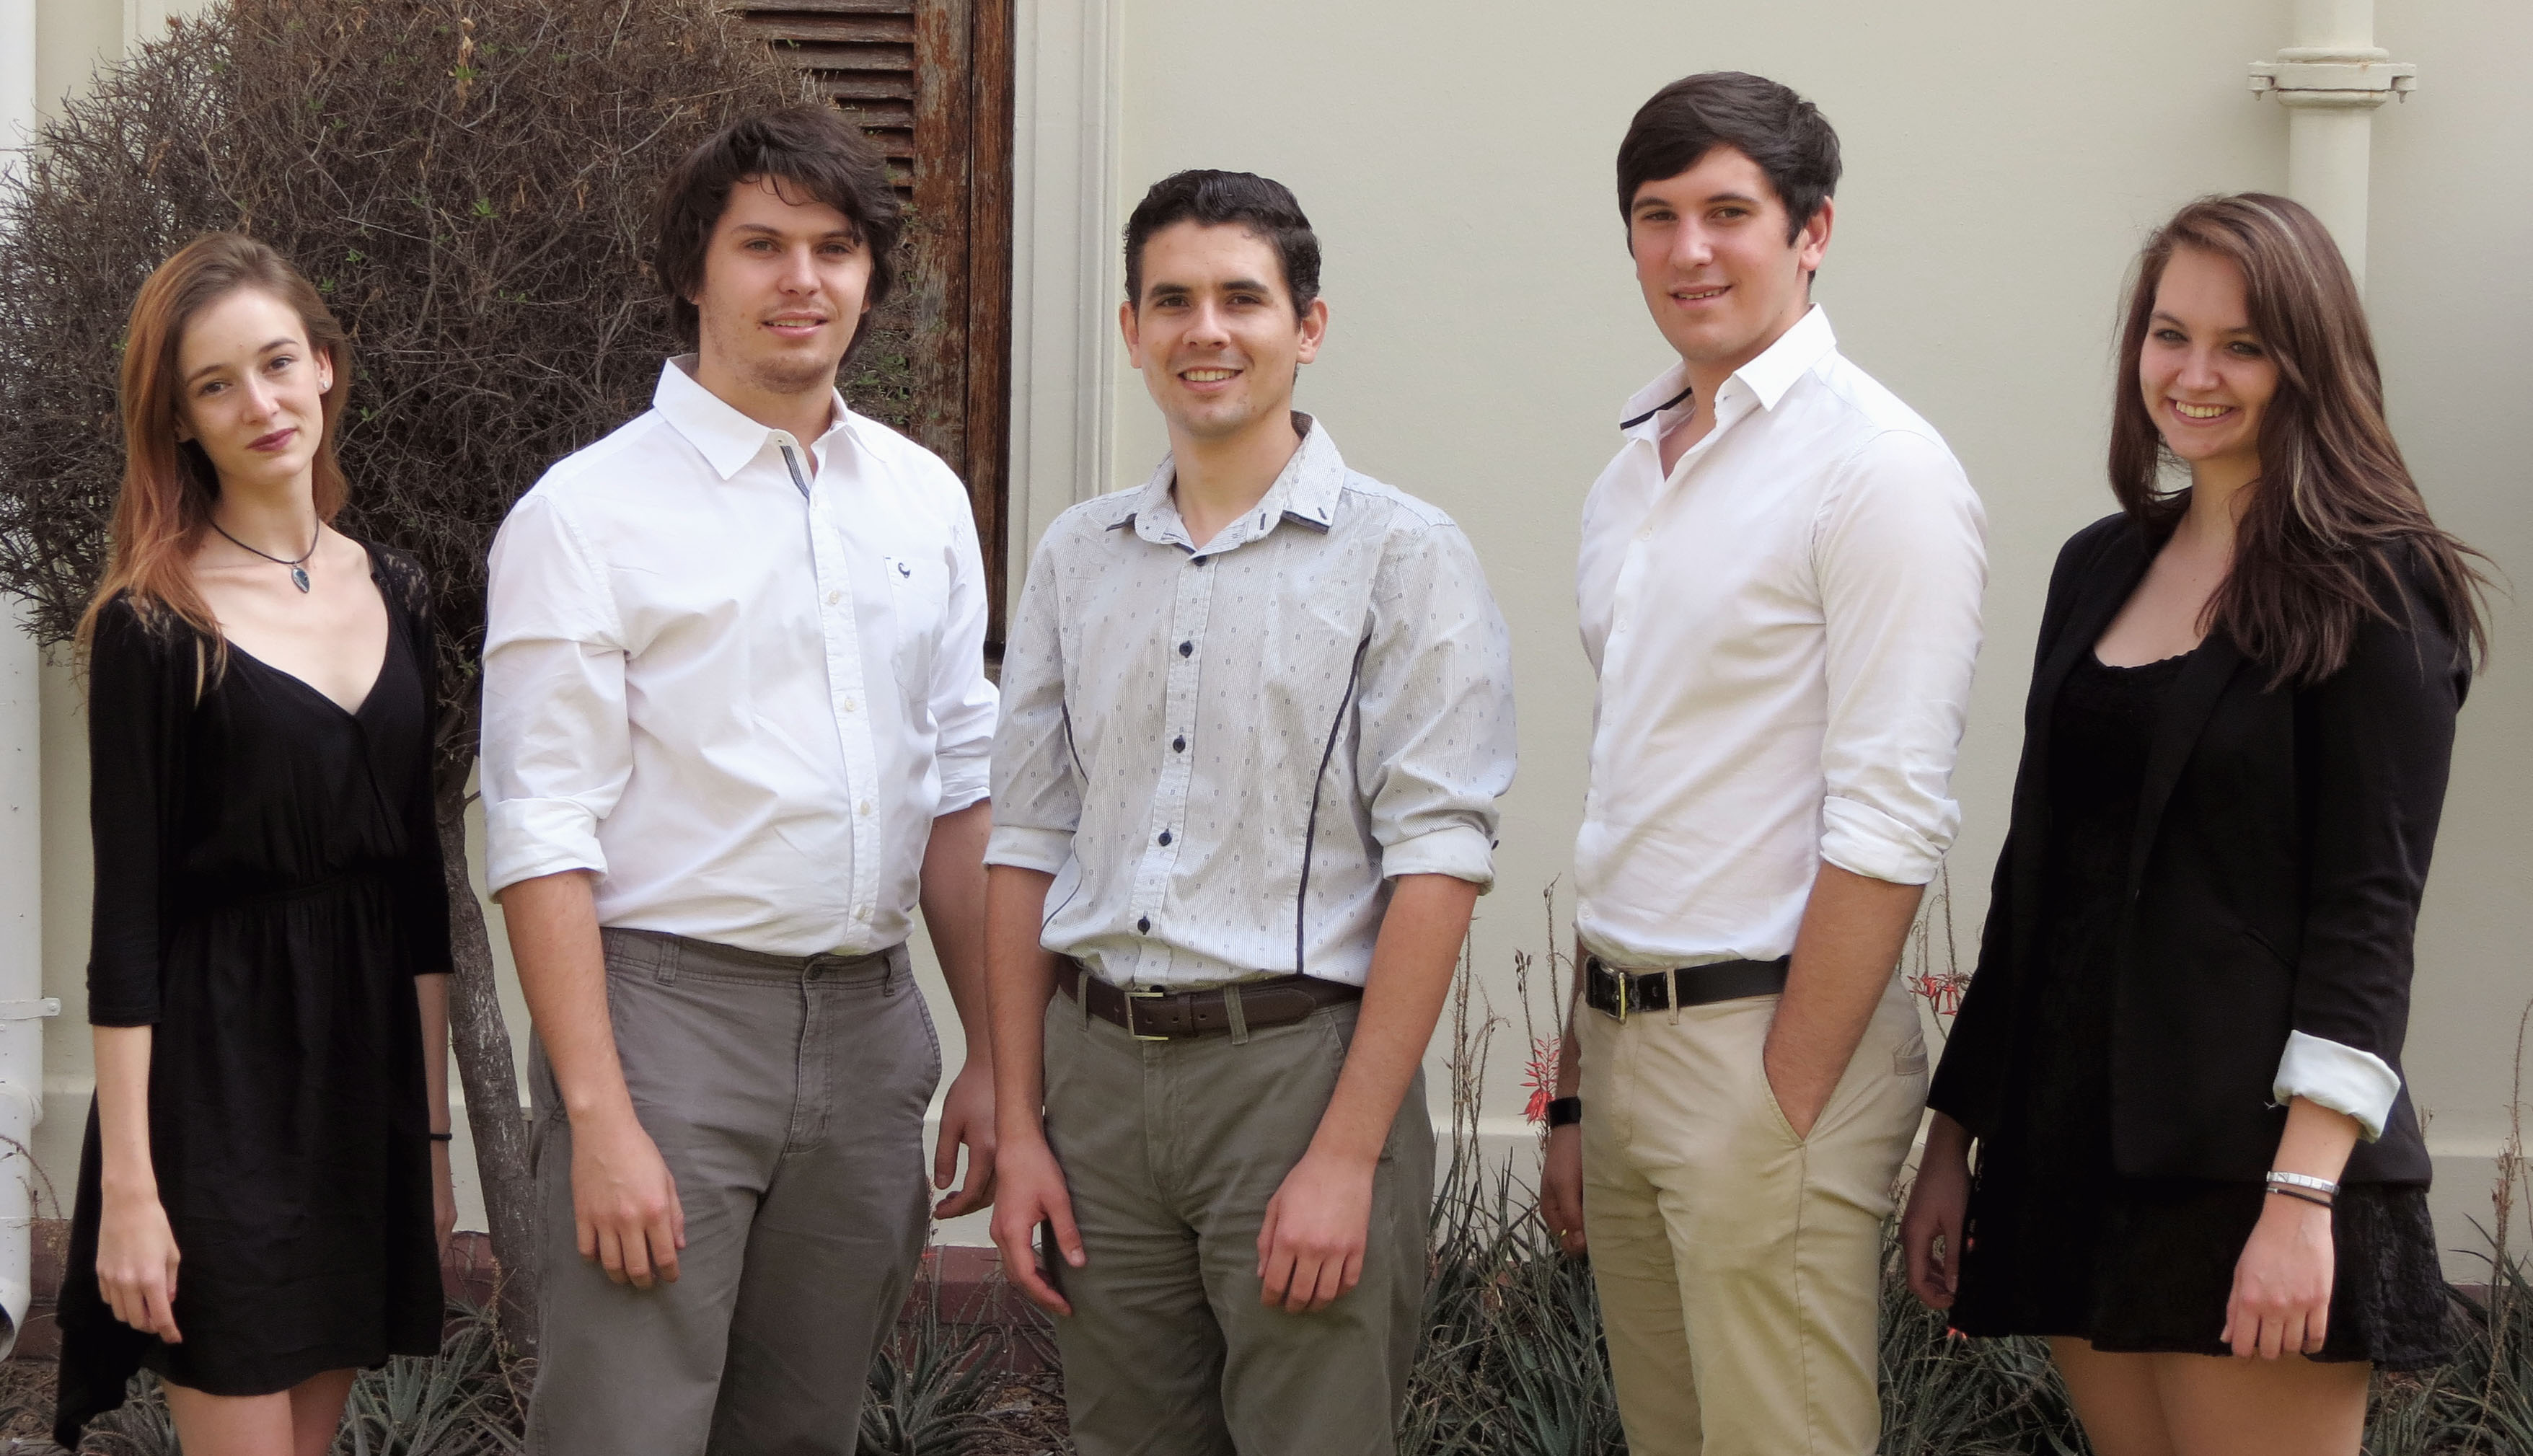
\includegraphics[width=0.9\textwidth]{team.jpg}};
            \node[fit=(pict),rounded corners=.55cm,inner sep=2pt]{};
         \end{tikzpicture}

         \par\vspace{1cm}
         \date{}
         \author{}
         \title{}
         \centering
         \textbf{Authors:}\\
         Mia Gerber\\
         Matthew Perry\\
         Wanrick Willemse\\
         Duart Breedt\\
         Linda Potgieter\\
      }
   \end{titlepage}
   \maketitle
   \tableofcontents
   \newpage
   
   \section{Project Description}
The scope of the project includes developing a \textbf{web interface}, \textbf{Android application}, and \textbf{iOS application}.\\\\
The entire application will be built with the \textbf{Ionic Framework}. This will allow for simple multi-platform development including Android and iOS devices. Furthermore, it will ensure the application’s web interface and mobile application have a uniform interface design.\\\\
We plan to use \textbf{ngCordova}’s geolocation functionality, which integrates natively with the Ionic Framework, to track users who are using the application. The user location’s will be viewable by farmers through either using the web interface and the \textbf{Google Static Map API} or through the mobile application and the \textbf{Google Maps Android API}. \\\\
Statistical and analytical data will be visualized with either the \textbf{Chart.js} API or \textbf{Plotly.js} API. This will allow the users to specify what type of graphical representation they would like to use view the gathered data as well as which data to visualize. Furthermore, \textbf{Math.js} will be used to calculate and gather relevant data. 
A server will need to be set up to save user data and productivity data. The majority of the MEAN stack is the preferred solution. \\\\
Therefore, \textbf{Node.js} will be used as the server which the mobile application as well as web interface will query. \textbf{Express.js} will be used as the server-side framework. \textbf{Jade.js} might be used as a templating engine. \textbf{Angular.js} will be a data-binding client-side solution. \textbf{MongoDB} will be the database which Node.js will query. MongoDB will be best since the application and web interface is run in a largely JSON and JavaScript environment.\\\\
We plan to have a dedicated admin user who can update the farm data such as produce types, locations, and location/crop boundaries. This will allow the application to be scaled if, for instance, the farm grows without having to redevelop the application or completely redraw the map. This will ensure robustness and flexibility in a demanding farm environment.\\\\
The application will be developed with the user in mind, therefore it will have a clear and simple design with easy to understand visual metaphors. We will ensure the interaction is designed in such a way to provide users with an increase in productivity and an experience of ease-of use.   

\subsection{Deployment Diagram}
\begin{center}
	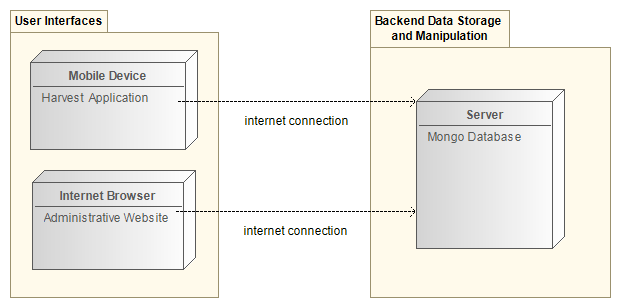
\includegraphics[width=0.5\linewidth]{deployment.png}
\end{center}

\section{Development Methodologies}
\subsection{Interaction between development team and client}

\textnormal First and foremost, we believe the client to be the expert, we are merely helping to create
			a system to supplement their already existing domain knowledge. In the case of Subtrop, domain knowledge will consist of typical work hours for farm workers, size of orchards, seasonal influences on crop yields and so forth, which will be acquired during our first meeting if our team is chosen for your project.
			\\ \\
			Moving more into the realm of software engineering, as a team we plan on strictly adhering 
			to Agile Principles. Clients will not only be queried for information but involved as much
			as possible in the testing of early prototypes so that their feedback can be integrated and 
			used as a guide for future releases.
			\\ \\
			Lastly, it is important to us that we as developers and you as our client at Subtrop both 
			agree on a scope for the project, requirements can and probably will change but in order
			to provide the best quality product in the time-frame given we need to first create a checklist of features to be implemented and continually refer back to them to ensure we are not going off scope.
				

\subsection{Interaction between members of development team}

\parbox{\textwidth}{ We decided on applying a SCRUM methodology in order to structure how teamwork will occur for
			this project, this is a faster, more intensely iterative approach to controlling workflow.
			We are using Slack and ZenHub (in conjunction with Github) to ensure that team members are aware of each other even when we are not physically together and are alerted when work is either available or completed.\\}
			Meetings will be held once a week regardless of whether there is a problem with
			the project or not, each meeting will require that each team member give a small summary
			of what work they had done that week, this enforces accountability. Working in weekly "sprints" also optimizes predictability and minimizes risk (if something does go wrong it is only a week's worth of work lost, not a whole month)\\\\
			As a team we are going to be adhering to a practice called "pair-programming" which is essentially two or more people working on the same piece of code or feature in order to maximize the chances of bugs being discovered and minimize the time required to get a feature ready for production. 
			\\ \\ 

	\newpage
	\section{Our Team}
		\parbox[c][4cm]{4cm}{\tikz\node[circle,draw,minimum size=3.5cm, 
			path picture={
               \node at (path picture bounding box.center){
                   
\includegraphics[width=3.5cm]{mia.jpg}
               };
           }]{};
		}
		\parbox[c][4cm]{10cm}{\subsection*{Mia Gerber}B.IS Multimedia}\\\\
Logical thinking and reasoning has always come naturally to me, I enjoy being posed a question or problem and then left to use the tools at my disposal to answer and/or solve it.\\\\
I am stubborn in the pursuit of success, which leads to many hours being sunk into troubleshooting if a product or deliverable does not meet all the requirements.\\\\
I am skilled in both the technical and creative side of development, in other words, formulating somewhat unconventional solutions and then executing them in a professional manner.\\\\
I believe that my team members and I are capable of making this project a success through our already existing abilities as well as sheer tenacity.\\\\
		\textbf{\small Experience and Project:}\\
		University of Pretoria’s EBIT Week IT team\\
		eCommerce website (both front and backend development) as undergraduate project\\
		Teaching Assistant for the Computer Science department\\\\
		\parbox{\textwidth}{
			\textbf{\small Relevant skills:}
			\begin{itemize}\itemsep0em
				\item Programming Languages:
				\begin {itemize}\itemsep0em
					\item C++
					\item C
					\item C\#
					\item Java
					\item x86 Assembly Language
					\item Javascript
					\item JQuery
					\item Actionscript 3.0
				\end {itemize}
				\item Markup Languages:
				\begin {itemize}\itemsep0em
					\item XML
					\item HTML
					\item JSON
					\item CSS
					\item Bootstrap
				\end {itemize}
				\item Frameworks:
				\begin {itemize}\itemsep0em
					\item MEAN stack development
					\begin {itemize}\itemsep0em
						\item Node.js
						\item Angular.js
						\item Express.js
						\item MongoDB
					\end {itemize}
					\item LAMP stack development
					\begin {itemize}\itemsep0em
						\item MySQL
						\item PostgreSQL
						\item PHP
					\end {itemize}
				\end {itemize}
				\item Software:
				\begin {itemize}\itemsep0em
					\item Adobe Creative Suite
					\item Modelio
				\end {itemize}
			\end{itemize}
		}
		\newpage
		\parbox[c][4cm]{4cm}{\tikz\node[circle,draw,minimum size=3.5cm, 
			path picture={
               \node at (path picture bounding box.center){
                   
\includegraphics[width=3.5cm]{matthew.jpg}
               };
           }]{};
		}
		\parbox[c][4cm]{10cm}{\subsection*{Matthew Perry}B.IT}\\\\
		I am passionate about software development. Being able to write code to solve a problem excites me. I am driven to be able to learn new technologies and be able to use them to create software and solve problems. I am a critical thinker that thrives when given something complex to assess and work on.
I am able to work well under pressure and ensure that the final result exceeds expectations. I can adapt to the situation so that I can perform at my peak. Learning and gathering experience are very important aspects in my life.\\\\
		\textbf{\small Experience and Project:}\\
		HCI task to redesign an app to improve user experience.\\
		Programmed an FPGA board using VHDL.\\\\
		\parbox{\textwidth}{
			\textbf{\small Relevant skills:}\\
			\parbox{5cm}{
				\begin{itemize}\itemsep0em
					\item OOP
					\begin {itemize}\itemsep0em
						\item C++
						\item Java
						\item Python
						\item Javascript
					\end {itemize}
				\end {itemize}
			} 
			\parbox{5cm}{
				\begin{itemize}\itemsep0em	
					\item Web Development
					\begin {itemize}\itemsep0em
						\item HTML
						\item PHP
						\item NodeJS
						\item SQL
						\item MongoDB
					\end {itemize}
				\end {itemize}
			}
			\begin{itemize}\itemsep0em	
				\item C
				\item Android Studio
				\item Hardware Descriptive Language: VHDL
				\item Cisco CCNA 6.0 and CCNP Route qualifications
				\item GIS (ArcGIS, QGIS)
			\end{itemize}
		}
		\newpage
		\parbox[c][4cm]{4cm}{\tikz\node[circle,draw,minimum size=3.5cm, 
			path picture={
               \node at (path picture bounding box.center){
                   
\includegraphics[width=3.5cm]{wanrick.jpg}
               };
           }]{};
		}
		\parbox[c][4cm]{10cm}{\subsection*{Wanrick Willemse}B.IS Multimedia}\\\\
		I’ve always enjoyed finding a solution to a challenge. I believe that anything can be overcome if it is approached systematically and with determination.\\\\
Meticulous design and thorough planning should be at the forefront of tackling a problem. I try to establish a vision and use it as a roadmap when creating something. I consider a product successful when I can see it is of a high standard.\\\\
I am adaptable and can function well under pressure. When it comes to my work, there is no settling for second best.\\\\
Developing high-quality software expects no less.\\\\
		\textbf{\small Experience and Project:}\\
		7 years work experience at a pathology company\\
		eCommerce website as undergraduate project\\
		Tutor for first year webdesign and second year Visual Design\\\\
		\parbox{\textwidth}{
			\textbf{\small Relevant skills:}
			\begin{itemize}\itemsep0em
				\item OOP and Procedural programming in: C++, C, Java, PHP, Python and JavaScript
				\item Web Development: HTML, CSS, Bootstrap, MEAN and LAMP stack
				\item XML, JSON and WebGL
				\item Adobe Suite, HCI, UX and UI design
			\end{itemize}
		}
		\newpage
		\parbox[c][4cm]{4cm}{\tikz\node[circle,draw,minimum size=3.5cm, 
			path picture={
               \node at (path picture bounding box.center){
                   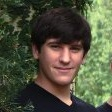
\includegraphics[width=3.5cm]{duart.jpg}
               };
           }]{};
		}
		\parbox[c][4cm]{10cm}{\subsection*{Duart Breedt}B.IS Multimedia}\\\\
		I take pride in making all my work aesthetically pleasing and believe it is of the utmost importance that all user-centered products should have great UI and UX design.\\\\
I think of myself as a perfectionistic completionist. Characteristically, I work persistently on any endeavour I undertake until I have produced a quality product I am proud of.\\\\
\parbox{\textwidth}{I find that if I am not learning, I am bored. Therefore, I strive to seek out challenges which push my limits and force me to contend with steep learning curves.\\}
I strongly believe that if you ever wish to be great at what you do you should ensure you are never the smartest person in the room. People are vessels of knowledge and will teach you more than you would like to know if you let them.\\\\
		\textbf{\small Experience and Projects (Please see my LinkedIn and GitHub for more detail):}\\
		Developed a website for Caelum Technologies\\
		Developing a website for the National Field Trial Association\\
		Developing a website for TallTrees Learning Community\\
		\href{http://77-breedt.000webhostapp.com}{Developed an ecommerce website as an undergraduate based project}\\\\
		\parbox{\textwidth}{		
			\textbf{\small Relevant skills:}
			\begin{itemize}\itemsep0em
				\item Object-Oriented Programming
				\item Java
				\item C++
				\item XML
				\item JSON
				\item Web Development:
				\begin {itemize}\itemsep0em
					\item HTML
					\item CSS
					\item Bootstrap
					\item Javascript
					\item JQuery
					\item MEAN stack (NodeJS, MongoDB, AngularJS)
					\item LAMP stack (PHP, SQL)
				\end {itemize}
				\item Design principles (UI, UX, HCI)
				\item Visual Design
				\item Adobe Creative Suite

			\end{itemize}
		}
		\newpage
		\parbox[c][4cm]{4cm}{\tikz\node[circle,draw,minimum size=3.5cm, 
			path picture={
               \node at (path picture bounding box.center){
                   
\includegraphics[width=3.5cm]{linda.jpg}
               };
           }]{};
		}
		\parbox[c][4cm]{10cm}{\subsection*{Linda Potgieter}B.IT}\\\\
		I am always up for a challenge. Nothing great is worth achieving by taking the easy way out.. I am always analyzing the problem to ensure I find the most effective but easiest to understand solution.\\\\
I am always willing to find a solution to a problem on my own, but I know when I need to ask for assistance. Struggling alone is not an option when project quality is at stake. Strong believer in the use and creation of complete and concise documentation for any project. \\\\
I perform well under pressure, but ensure the pressure placed on myself with regards to my studies is at minimum by setting milestones and achieving them within a set timeframe. No one likes sloppy last minute work, and clients deserve more than that, even if it is only a teaching assistant assessing the work.\\\\
		\textbf{\small Experience and Project:}\\
		Redesign of mobile application to comply with HCI standards as undergraduate project.\\\\
		\parbox{\textwidth}{
			\textbf{\small Relevant skills:}
			\begin{itemize}\itemsep0em
				\item Java
				\item Python
				\item C++
				\item x86 Assembly Language 
				\item JSON
				\item Web development
				\begin {itemize}\itemsep0em
					\item HTML
					\item CSS
					\item Bootstrap
					\item XML
					\item JavaScript
					\item JQuery
					\item MEAN Stack
					\begin {itemize}\itemsep0em
						\item AngularJS
						\item NodeJS
						\item MongoDB
						\item ExpressJS
					\end {itemize}
					\item LAMP stack
					\begin {itemize}\itemsep0em
						\item PHP
						\item SQL (MySQL and MSQL)
					\end {itemize}
				\end {itemize}
				\item Design principles
				\item Human Computer Interaction design
				\item User interface design
				\item User experience design
				\item Other 
				\begin {itemize}\itemsep0em
					\item Genome analysis programs 
					\begin {itemize}\itemsep0em
						\item MEGA 6.06
						\item Mothur
						\item MCRobot
					\end {itemize}
				\end {itemize}
			\end{itemize}
		}

\end{document}
